\section{One manoeuvre}\label{sec:one}

\subsection{Statement}
Recall $X(\psi)=d_b\cos\psi-\Rm\sin\psi$ and $Y(\psi)=\Rm\cos\psi-b\sin\psi$.
Let
\[
  \varepsilon_b=r-\Rp=\sqrt{d_b^2+\Rp^2}-\Rp
\]
be the \emph{rear swing}: the amount by which the rear curb-side corner dips below its starting height when a car parked level drives forward with full left lock.
When $H<\ell$ (which follows from \ref{A:fit} below), let $\psi_b\in(0,\pi/2)$ be defined by $\sin\psi_b=H/\ell$, and put $c_2=2b/\sin\psi_b$.
Since $Y$ is strictly decreasing on $[0,\pi/2]$, the equation
\begin{equation}\label{eq:psid}
  Y(\psi_d)=r-H
\end{equation}
has a unique solution $\psi_d\in[0,\pi/2)$ as soon as $Y(0)=\Rm\ge r-H$, i.e.\ as soon as $m\ge\varepsilon_b$.

\begin{assumption}\label{ass:one}
\leavevmode
\begin{enumerate}[label=(A\arabic*),nosep]
\item\label{A:db} $d_b<b$, $\Rp^2>bd_b$, and $m\ge\varepsilon_b$;
\item\label{A:fit} $H<b$, $H<\Rm+d_b$, $\cos\psi_b>m/w$, $\psi_{\rm fit}<\beta$, $\Rp\cos\psi_{\rm fit}>\max(H,\Rm)$ and $\Rm\ge d_b\tan(\psi_{\rm fit}/2)$;
\item\label{A:nose} $2Rb>w\rho$, $wb>m\rho$ and $b\rho>H\Rp$;
\item\label{A:curbcase} $(\Rp^2-bd_b)/r\ge r-H$;
\item\label{A:min} $\cos\psi_d\sqrt{b^2+2Rw}>\Rm\sin\psi_d+b$ and
 \[
   b\cos\psi_{\rm fit}\,\big(2Y(\psi_{\rm fit})+c_2\big)>2(\Rm+d_b\sin\psi_{\rm fit})\sqrt{\rho^2+c_2\,\big(r-H-Y(\psi_{\rm fit})\big)};
 \]
\item\label{A:end} $r-d_b\ge H$ and $X(\psi_d)\ge0$;
\item\label{A:far} $d_b\cos\psi_{\rm fit}-\Rp\sin\psi_{\rm fit}+\rho\ge\Lambda_1$ and $B_{\rm back}\ge\Lambda_1$, where $\Lambda_1$ is defined in \eqref{eq:Lambda1def} below and $B_{\rm back}$ in \eqref{eq:Bback}.
\end{enumerate}
\end{assumption}

These are mild ``realistic car'' inequalities.
\Cref{app:assumptions} checks them for the typical car of \cref{tab:values} and on a grid of 1280 parameter sets covering passenger cars, with $m=w/10$.
They fail mainly when $m<\varepsilon_b$ (an unusually long rear overhang combined with a very tight turning circle), and otherwise only for very short and wide cars.
Only \ref{A:db} and \ref{A:end} enter the upper bound; the other conditions serve the lower bound.

\begin{theorem}\label{thm:one}
Under \cref{ass:one},
\begin{equation}\label{eq:Lambda1def}
  \Lmin(1)=\Lambda_1:=X(\psi_d)+\sqrt{\rho^2-(r-H)^2}.
\end{equation}
Equivalently, with $\varsigma=r-H$ and $s_0^2=b^2+\Rm^2$,
\[
  \Lambda_1=\frac{\ell\,\Rm\,\varsigma+(bd_b-\Rm^2)\sqrt{s_0^2-\varsigma^2}}{s_0^2}+\sqrt{\rho^2-\varsigma^2}.
\]
The infimum is attained.
An optimal exit starts from the parked configuration $q_d$ with heading $\psi_d$ whose lane-side corners touch the line $y=H$ and the car behind ($\cFL_y=H$, $\cRL_x=0$).
It drives forward with full left lock, during which the front curb-side corner grazes $\Qf$ and the rear curb-side corner grazes the curb, and then straightens with full right lock.
\end{theorem}

The closed form follows from \eqref{eq:psid}: writing $(\Rm,b)=s_0(\cos\chi,\sin\chi)$ we get $\psi_d+\chi=\arccos(\varsigma/s_0)$, hence
$\cos\psi_d=(\varsigma\Rm+b\sqrt{s_0^2-\varsigma^2})/s_0^2$ and $\sin\psi_d=(\Rm\sqrt{s_0^2-\varsigma^2}-\varsigma b)/s_0^2$.

\begin{corollary}[classical formula]\label{cor:classical}
Under \cref{ass:one}, if $m=\varepsilon_b$, then $\psi_d=0$ and $\Lmin(1)=d_b+\sqrt{b^2+2Rw}=d_b+\sqrt{(d_w+d_f)^2+(R+\tfrac w2)^2-(R-\tfrac w2)^2}$.
For $m>\varepsilon_b$ the value $\Lambda_1$ is strictly smaller.
\end{corollary}
\begin{proof}
For $m=\varepsilon_b$ we have $r-H=\Rm$, so $\psi_d=0$, $X(0)=d_b$ and $\rho^2-\Rm^2=b^2+2Rw$.
If $m>\varepsilon_b$, then $\psi_d>0$, and the first inequality of \ref{A:min} shows that $\psi\mapsto X(\psi)+\sqrt{\rho^2-Y(\psi)^2}$ is strictly decreasing on $[0,\psi_d]$; hence $\Lambda_1$ is smaller than its value at $\psi=0$, which is the classical length.
\end{proof}

For the typical car of \cref{tab:values}: $\varepsilon_b=0.069<m=0.18$, $\psi_d=0.0314$ rad $=1.80^\circ$, $\Lambda_1=5.833$~m, while the classical value is $5.861$~m.
In driving terms, the optimal \emph{parking} manoeuvre (time-reversed) reverses with full right lock, then reverses with full left lock, and stops while the car is still turned $1.8^\circ$ nose-up (see \cref{fig:one}).

\begin{figure}[ht]
\centering
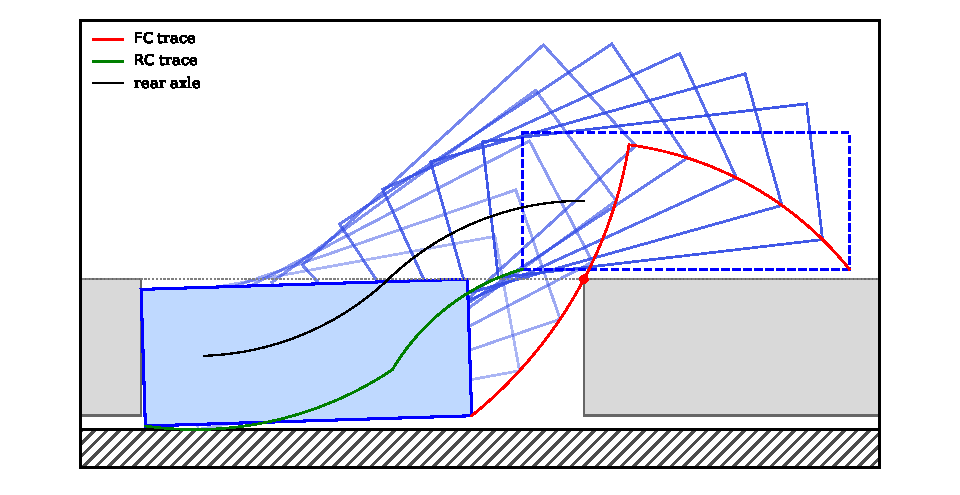
\includegraphics[width=0.85\textwidth]{figures/fig_one.pdf}
\caption{The optimal single manoeuvre for the typical car, drawn as an exit: full left lock from $q_d$ (filled) up to the heading $0.76$ rad, then full right lock to the level lane position (dashed).
Read backwards, it is the parking manoeuvre: reverse with right lock, then with left lock.
The front curb-side corner (red trace) grazes $\Qf$; the rear curb-side corner (green trace) grazes the curb.}
\label{fig:one}
\end{figure}

\subsection{The upper bound}

\begin{proposition}\label{prop:one-upper}
Assume \ref{A:db} and \ref{A:end}, and let $L=\Lambda_1$.
Let $q_d=(P,\psi_d)$ with $P=\big(d_b\cos\psi_d+\tfrac w2\sin\psi_d,\ H-b\sin\psi_d-\tfrac w2\cos\psi_d\big)$.
Then $q_d$ is parked.
The exit consisting of forward full left lock from heading $\psi_d$ to $\pi/2$, followed by forward full right lock from $\pi/2$ to $0$, is free and ends in a lane configuration.
Hence $\Lmin(1)\le\Lambda_1$.
\end{proposition}

\begin{proof}
For $q_d$ the left centre is
\[
  C=P+R\n(\psi_d)=\big(X(\psi_d),\,H+Y(\psi_d)\big)=\big(X(\psi_d),\,r\big)
\]
by \eqref{eq:psid}.
By construction $\cFL_y=H$ and $\cRL_x=0$.

\emph{$q_d$ is parked.}
The highest point is $\cFL$ and the leftmost is $\cRL$, so the footprint lies in $\{y\le H\}\cap\{x\ge0\}$.
By \eqref{eq:RCy} the lowest point satisfies $\cRC_y=r-r\cos(\psi_d-\beta)\ge0$.
For the front, $\cFC=C+\rho\,\e(\psi_d-\gamma)$ lies on the circle of radius $\rho$ about $C$, below the height $H$.
The point of that circle at height $H$ on its right half is $(\Lambda_1,H)=\Qf$, because $C_y-H=r-H$ and $\Lambda_1-C_x=\sqrt{\rho^2-(r-H)^2}$.
Moving along the lower right quarter of the circle towards $\Qf$ increases $x$, so $\cFC_x<L$.
Since $\cFC$ is the rightmost point, the footprint lies in $\{x\le L\}$, hence in $\Free$.

\emph{First arc.}
During forward full left lock the footprint rotates counter-clockwise about the fixed point $C$ through the angle $\pi/2-\psi_d$ (\cref{sec:toolkit}).
\begin{itemize}[nosep]
\item \emph{Front.} By \cref{lem:disk} the footprint stays in the closed disk $D$ of radius $\rho$ about $C$.
If $p=(p_x,p_y)\in\Of$, then $p_x-C_x>L-C_x\ge0$ and $C_y-p_y>C_y-H\ge0$, so $|p-C|^2>|\Qf-C|^2=\rho^2$.
Thus $\Of\cap D=\emptyset$.
\item \emph{Rear and curb.} At the start every point of the footprint lies strictly below $C$, since $y\le H<r=C_y$ by \ref{A:end}.
Consider a point at polar angle $\vartheta_0\in(\pi,2\pi)$ about $C$; during the arc its angle is $\vartheta_0+t$ with $t\in[0,\pi/2-\psi_d]$.
\begin{itemize}[nosep]
\item If $\vartheta_0\in(\pi,3\pi/2]$, the angle stays in $(\pi,2\pi)$, where $\cos$ is increasing, so the point moves right and keeps $x\ge0$.
\item If $\vartheta_0\in(3\pi/2,2\pi)$, the angle stays in $(3\pi/2,5\pi/2)$, where $\cos\ge0$, so $x\ge C_x=X(\psi_d)\ge0$.
\end{itemize}
Hence no point enters $\Or$.
For the curb, points with $\vartheta_0\in(3\pi/2,2\pi)$ only rise.
A point with $\vartheta_0\in(\pi,3\pi/2]$ has body coordinates $(u,v)$ with $u\cos\psi_d-(v-R)\sin\psi_d\le0$, hence $u\le0$.
Its distance from $C$ is therefore at most $\sqrt{d_b^2+\Rp^2}=r$, so its height never drops below $C_y-r=0$.
\end{itemize}

\emph{End of the first arc.}
At heading $\pi/2$ we have $P=C+(R,0)$, and a body point $(u,v)$ sits at $C+(R-v,u)$.
Its height is $C_y+u\ge r-d_b\ge H$ by \ref{A:end}, so the car is in the lane.

\emph{Second arc.}
Forward full right lock rotates the car clockwise about $C'=C+(2R,0)$.
All points have $x\le C_x+R+w/2<C'_x$ when the arc starts.
Along a clockwise rotation, the height of each point is a unimodal function of time (it rises until the point passes the top of its circle).
It therefore stays above the minimum of its initial and final heights.
The final configuration is level with rear axle at height $C_y+R$, so all its points have $y\ge r+\Rm>H$.
Hence the car remains in the lane and ends parallel to the curb.
\end{proof}

\begin{remark}
The quarter turn is chosen for ease of proof.
Any switching heading $\alpha\ge\alpha_{\min}$ between left and right lock gives a valid exit.
For the typical car the binding constraint is that the final level position lies in the lane, $r+\Rm-2R\cos\alpha\ge H$, so $\alpha_{\min}=\arccos\big((r+\Rm-H)/(2R)\big)=0.734$ rad ($42.0^\circ$); a numerical collision check finds no other active constraint.
These are the familiar S-shaped parking paths: in forward time one reverses with right lock and then with left lock.
\end{remark}

\subsection{Lower bound for forward exits}

\begin{proposition}\label{prop:one-forward}
Suppose that \cref{ass:one} holds.
If a forward manoeuvre leads from a parked configuration $q_0$ with $|\psi(0)|\le\psi_{\rm fit}$ to a lane configuration through free configurations, then $L\ge\Lambda_1$.
\end{proposition}

\begin{proof}
Suppose $L<\Lambda_1$.
Write $q(s)=(P(s),\psi(s))$, $s\in[0,S]$, and let $C(s)$, $C'(s)$ be the turning centres.

\emph{Step 1: the crossing time.}
At the end the whole car lies in $\{y\ge H\}$, so $\cFC_y(S)\ge H$.
At the start $\cFC_y(0)=\cFL_y(0)-w\cos\psi(0)<H$.
Let $\tau=\min\{s:\cFC_y(s)=H\}$.

\emph{Step 2: heading bounds on $[0,\tau]$.}
Let $s_*\le\tau$ be the supremum of the times $t\le\tau$ such that $-\gamma<\psi<\psi_b$ on $[0,t)$; it is positive because $|\psi(0)|\le\psi_{\rm fit}<\min(\gamma,\psi_b)$.
Indeed $\psi_{\rm fit}<\beta<\gamma$ by \ref{A:fit} and \ref{A:db} (the second inequality is equivalent to $\Rp^2>bd_b$), and $\ell\sin\psi_{\rm fit}=H-w\cos\psi_{\rm fit}<H$ gives $\psi_{\rm fit}<\psi_b$.
In particular $\cos\psi_{\rm fit}>\cos\psi_b>m/w$ by \ref{A:fit}, so \cref{lem:parked} applies.
We first collect consequences valid on $[0,s_*)$.
\begin{itemize}
\item[(i)] Whenever $\psi\in[0,\pi/2]$ the lowest point is $\cRC$, so $P_y\ge d_b\sin\psi+\tfrac w2\cos\psi$ and hence $\cFC_y\ge\ell\sin\psi$.
For $s<\tau$ this gives $\ell\sin\psi<H$, i.e.\ $\psi<\psi_b$ whenever $\psi\in[0,\pi/2]$.
\item[(ii)] If $\psi(s)\in[0,\psi_b)$ then $P_y=\cFC_y-b\sin\psi+\tfrac w2\cos\psi<H+\tfrac w2$.
Since $P_y'=\sin\psi$ and $\psi>-\gamma>-\pi$, $P_y$ decreases on intervals where $\psi<0$; also $P_y(0)<H+w/2$.
Hence $P_y<H+w/2$ on $[0,s_*)$, and by continuity $P_y(s_*)\le H+w/2$.
\item[(iii)] On $[0,s_*)$ we have $\cos\psi>0$, so by \cref{lem:drift} $C'_x$ is non-decreasing on $[0,s_*]$.
Moreover $C'_x(0)=P_x(0)+R\sin\psi(0)\ge d_b\cos\psi_{\rm fit}-\Rp\sin\psi_{\rm fit}$.
For $\psi(0)\ge0$ this follows from \cref{lem:parked}(a), and for $\psi(0)<0$ from \cref{lem:parked}(b).
\end{itemize}
Now suppose $\psi(t)=-\gamma$ for some $t\le s_*$ (by continuity this is the only way $-\gamma<\psi$ can fail at $s_*$).
By \cref{lem:polar}, $\cFL(t)=C'(t)+(\rho,0)$, so by (iii) and \ref{A:far},
\[
  \cFL_x(t)\ge d_b\cos\psi_{\rm fit}-\Rp\sin\psi_{\rm fit}+\rho\ge\Lambda_1>L .
\]
Its height is $\cFL_y=P_y-R\cos\gamma\le H+\tfrac w2-\tfrac{Rb}\rho<H$ by (ii) and \ref{A:nose}.
If $\cFL_y>m$, then $\cFL\in\Of$.
Otherwise $\cFC_y=\cFL_y-w\cos\gamma\le m-wb/\rho<0$ by \ref{A:nose}, and the car meets the curb.
Both are impossible.
Likewise $\psi(s_*)=\psi_b$ with $s_*<\tau$ is excluded by (i).
Hence $s_*=\tau$, and $-\gamma<\psi(\tau)\le\psi_b$.

\emph{Step 3: $\psi(\tau)\in[0,\psi_b]$.}
If $\psi(\tau)\in(-\gamma,0)$, the lowest point is $\cFC$, at height $H$.
Then $P_y(\tau)=H+b|\sin\psi|+\tfrac w2\cos\psi$, while $P_y(\tau)\le H+w/2$ by (ii).
This gives $\tan(|\psi|/2)\ge 2b/w>1$ (note $2b>w$ by \ref{A:nose}), contradicting $|\psi|<\pi/2$.

\emph{Step 4: $\cFC_x(\tau)\le L$.}
For $s<\tau$ close to $\tau$ the height of $\cFC(s)$ lies in $(m,H)$.
Since $\cFC(s)\notin\Of$, $\cFC_x(s)\le L$, and we let $s\uparrow\tau$.

\emph{Step 5: $\Qf$ stays ahead of the rear axle.}
We claim that for $s\in[0,\tau]$
\begin{equation}\label{eq:ahead}
  (\Qf-P)\cdot\e(\psi)\ \ge\ b-H\sin\gamma>0,\qquad\text{and}\qquad (\Qf-P)\cdot\e(\psi)\ge b\ \text{ if }\psi\ge0 .
\end{equation}
Write $(\Qf-P)\cdot\e=(L-\cFC_x)\cos\psi+(H-\cFC_y)\sin\psi+b$, and note $H-\cFC_y\ge0$.

If $\psi\ge0$ and $\cFC_y>m$, then $\cFC_x\le L$, and both terms are $\ge0$.
If $\psi\ge0$ and $\cFC_y\le m$, the front edge rises from $\cFC$ in direction $\n(\psi)$ to $\cFL$, with $\cFL_y=\cFC_y+w\cos\psi\in(m,H]$ by \ref{A:fit}.
Its point at height $m$ has $x\le L$, so $L-\cFC_x\ge-(m-\cFC_y)\tan\psi$.
Then $(L-\cFC_x)\cos\psi+(H-\cFC_y)\sin\psi\ge(H-m)\sin\psi=w\sin\psi\ge0$.

If $\psi<0$, the front edge rises from $\cFC$ in direction $\n(\psi)=(|\sin\psi|,\cos\psi)$ to $\cFL$, so $\cFC_x\le\cFL_x$.
If $\cFL_y\le m$ then $\cFC_y=\cFL_y-w\cos\psi<0$, which is impossible; here $w\cos\psi>w\cos\gamma=wb/\rho>m$ by \ref{A:nose}.
If $\cFL_y\in(m,H)$ then $\cFC_x\le\cFL_x\le L$.
If $\cFL_y\ge H$, the point of the front edge at height $H$ has $x\le L$, and it lies to the right of $\cFC$.
In all cases $\cFC_x\le L$, and $(H-\cFC_y)|\sin\psi|\le H\sin\gamma$ because $\cFC_y\ge0$ and $|\psi|<\gamma$.
The positivity of $b-H\sin\gamma=b-H\Rp/\rho$ is \ref{A:nose}.

\emph{Step 6: the corner is far from the centre at time $\tau$.}
At $\tau$, $\Qf=\cFC(\tau)+(\delta,0)$ with $\delta=L-\cFC_x(\tau)\ge0$.
In body coordinates of $q(\tau)$ the point $\Qf$ is $(b+\delta\cos\psi,\,-\tfrac w2-\delta\sin\psi)$, and $C$ is $(0,R)$.
As $\psi(\tau)\in[0,\pi/2)$,
\[
  |C(\tau)-\Qf|^2=(b+\delta\cos\psi)^2+(\Rp+\delta\sin\psi)^2\ \ge\ \rho^2 .
\]

\emph{Step 7: curb cost.}
By \cref{lem:distance} and \eqref{eq:ahead}, on $[0,\tau]$
\[
  \frac{\dd}{\dd s}|C-\Qf|^2=-2(1-R\psi')(\Qf-P)\cdot\e\le0,\qquad \frac{\dd C_y}{\dd s}=(1-R\psi')\sin\psi .
\]
If $\psi\in(0,\psi_b)$, then $(\Qf-P)\cdot\e\ge b\ge(b/\sin\psi_b)\sin\psi$.
If $\psi\le0$, then $\frac{\dd C_y}{\dd s}\le0$.
In both cases $\frac{\dd}{\dd s}\big(|C-\Qf|^2+c_2C_y\big)\le0$ with $c_2=2b/\sin\psi_b$.
Consequently, for every $t\in[0,\tau]$,
\begin{equation}\label{eq:curbcost}
  |C(0)-\Qf|^2\ \ge\ |C(\tau)-\Qf|^2+c_2\big(C_y(t)-C_y(0)\big)\ \ge\ \rho^2+c_2\big(C_y(t)-C_y(0)\big).
\end{equation}
The first inequality holds because $|C-\Qf|^2$ is non-increasing on $[t,\tau]$ and $|C-\Qf|^2+c_2C_y$ is non-increasing on $[0,t]$.

\emph{Step 8: the curb forces $C_y\ge r$ at some time.}
By \eqref{eq:RCy} and the curb, $C_y(s)\ge r\cos(\psi(s)-\beta)$ for all $s$.
If $\psi$ takes the value $\beta$ on $[0,\tau]$, this gives $C_y\ge r$ there.
Otherwise $\psi<\beta$ on $[0,\tau]$, because $\psi(0)\le\psi_{\rm fit}<\beta$.
In that case \eqref{eq:RCy} at $\tau$ gives $C_y(\tau)=H+\rho\sin(\gamma-\psi(\tau))\ge H+\rho\sin(\gamma-\beta)$, using $0\le\psi(\tau)<\beta<\gamma$ ($\beta<\gamma$ is equivalent to $\Rp^2>bd_b$).
Now $\rho\sin(\gamma-\beta)=(\Rp^2-bd_b)/r\ge r-H$ by \ref{A:curbcase}.
Either way some $t\in[0,\tau]$ has $C_y(t)\ge r$, and \eqref{eq:curbcost} yields
\[
  (L-C_x(0))^2+(C_y(0)-H)^2=|C(0)-\Qf|^2\ \ge\ \rho^2+c_2\big(r-C_y(0)\big)^+ .
\]
Moreover $C_x(0)\le P_x(0)+R\sin\psi_{\rm fit}\le L-b\cos\psi_{\rm fit}+\Rp\sin\psi_{\rm fit}<L$.
Here we used \cref{lem:parked}(c), and $\tan\psi_{\rm fit}<\tan\beta=d_b/\Rp<b/\Rp$.
Taking square roots, we obtain
\begin{equation}\label{eq:Phi}
  L\ \ge\ \Phi(q_0):=C_x(0)+\sqrt{\rho^2-(C_y(0)-H)^2+c_2\big(r-C_y(0)\big)^+}.
\end{equation}

\emph{Step 9: minimisation over parked configurations.}
$\Phi$ is increasing in $C_x$ and, on $\{C_y\ge H\}$, decreasing in $C_y$.
If $\psi(0)\in[0,\psi_{\rm fit}]$, \cref{lem:parked}(a) gives $C_x\ge X(\psi)$ and $H<\Rp\cos\psi_{\rm fit}\le\Rp\cos\psi\le C_y\le H+Y(\psi)$, using \ref{A:fit}; so $\Phi(q_0)\ge\varphi_{\rm c}(\psi(0))$ with
\[
  \varphi_{\rm c}(\psi):=X(\psi)+\sqrt{\rho^2-Y(\psi)^2+c_2\big(r-H-Y(\psi)\big)^+}.
\]
If $\psi(0)<0$, \cref{lem:parked}(b) gives $H<\Rp\cos\psi_{\rm fit}\le C_y\le H+\Rm$ and $C_x\ge d_b\cos\psi+\Rm|\sin\psi|\ge d_b$.
The last inequality is equivalent to $\Rm\ge d_b\tan(|\psi|/2)$, which holds by \ref{A:fit}.
Hence $\Phi(q_0)\ge\varphi_{\rm c}(0)$.
Finally $\psi_d\le\psi_{\rm fit}$, because $q_d$ is parked (\cref{prop:one-upper,lem:fit}), and $\varphi_{\rm c}$ is decreasing on $[0,\psi_d]$ and increasing on $[\psi_d,\psi_{\rm fit}]$.
On $[0,\psi_d]$ the penalty vanishes and the derivative of $X+\sqrt{\rho^2-Y^2}$ is at most
\[
  -\Rm\cos\psi_d+\Rm(\Rm\sin\psi_d+b)/\sqrt{b^2+2Rw}<0
\]
by \ref{A:min}.
On $[\psi_d,\psi_{\rm fit}]$ the derivative is positive by the second inequality of \ref{A:min}.
Hence $L\ge\varphi_{\rm c}(\psi_d)=X(\psi_d)+\sqrt{\rho^2-(r-H)^2}=\Lambda_1$, a contradiction.
\end{proof}

\subsection{Lower bound for reverse exits}

For a reverse exit we follow the height of the curb-side end of the rear axle, i.e.\ of the point $P-\tfrac w2\n$,
\[
  h=P_y-\tfrac w2\cos\psi\qquad(|\psi|<\pi/2).
\]
For a reverse manoeuvre, $h'=-\sin\psi\,(1-\tfrac w2\psi')$ with $1-\tfrac w2\psi'\in[\Rm/R,\Rp/R]$.
So $h$ increases only while the car points nose-down, and then the curb limits the rate of increase.
Let $\psi_n=\arcsin(H/b)$ and $c_\psi=\cos\psi_n$, and let $\psi_u\in(0,\pi/2)$ solve $\Rm(1-\cos\psi_u)+d_b\sin\psi_u=H$; it exists since $\Rm+d_b>H$.
Put $h_0=H-w\cos\psi_{\rm fit}$ and
\begin{equation}\label{eq:Bback}
  B_{\rm back}=b\cos\psi_{\rm fit}-\tfrac w2\sin\psi_{\rm fit}+\min\big(f_b(-\psi_n),f_b(\psi_u)\big)+c_\psi\frac{Rb}{\Rp}\log^+\frac{Hb}{\ell h_0},
\end{equation}
where $f_b(\psi)=d_b\cos\psi-\tfrac w2\sin\psi$.

\begin{proposition}\label{prop:one-reverse}
Assume \ref{A:fit}.
If a reverse manoeuvre leads from a parked configuration with $|\psi(0)|\le\psi_{\rm fit}$ to a lane configuration through free configurations, then $L\ge B_{\rm back}$.
\end{proposition}

\begin{proof}
Let $\tau_r$ be the first time at which $\cRC_y=H$.
It exists because $\cRC_y(0)<H$ and the car ends in the lane.
At the start, $h(0)\le H-w\cos\psi(0)\le h_0<H$, because the highest point of the parked car is at most $H$.

\emph{Heading bounds.}
Let $s_1$ be the first time with $|\psi|=\pi/2$, and work on $[0,\min(s_1,\tau_r))$.
\begin{itemize}[nosep]
\item On intervals with $\psi<0$ we have $\cRC_y=h+d_b|\sin\psi|<H$, so $h<H$.
On intervals with $\psi\ge0$, $h$ does not increase.
Hence $h<H$ throughout.
\item If $\psi\le0$, the lowest point is $\cFC$, with $\cFC_y=h-b|\sin\psi|\ge0$.
Hence $|\sin\psi|\le h/b<H/b$ and $\psi>-\psi_n$.
\item Let $I=(s_a,s_b)$ be a maximal interval on which $\psi>0$, and suppose $\psi$ first reaches $\psi_u$ at $t\in I$.
Since $|\psi'|\le1/R$,
\[
  \int_{s_a}^t\sin\psi\dd s\ \ge\ R\int_{s_a}^t\sin\psi\,|\psi'|\dd s\ \ge\ R\big(\cos\psi(s_a)-\cos\psi_u\big).
\]
Therefore $h(t)\le h(s_a)-\Rm(\cos\psi(s_a)-\cos\psi_u)$.
If $s_a>0$ then $\psi(s_a)=0$ and $h(s_a)<H$.
If $s_a=0$, then $h(0)\le H-w\cos\psi_{\rm fit}$ and $\cos\psi(0)\ge\cos\psi_{\rm fit}$, so $h(t)\le H-\Rp\cos\psi_{\rm fit}+\Rm\cos\psi_u<H-\Rm(1-\cos\psi_u)$ because $\Rp\cos\psi_{\rm fit}>\Rm$.
In both cases $h(t)<H-\Rm(1-\cos\psi_u)=d_b\sin\psi_u$.
This contradicts $\cRC_y(t)=h(t)-d_b\sin\psi_u\ge0$.
\end{itemize}
Thus $\psi\in(-\psi_n,\psi_u)\subset(-\pi/2,\pi/2)$ before $\min(s_1,\tau_r)$; hence $s_1>\tau_r$, and the bounds hold on $[0,\tau_r]$.

\emph{Gronwall.}
On intervals where $\psi<0$, we get $h'\le(\Rp/R)|\sin\psi|\le(\Rp/(Rb))\,h$.
Elsewhere $h$ does not increase.
Hence $h(\tau_r)\le h_0\exp\big(\tfrac{\Rp}{Rb}S_-\big)$, where $S_-$ is the total length of the intervals where $\psi<0$.
At $\tau_r$: if $\psi\le0$ then $H=\cRC_y=h+d_b|\sin\psi|\le h\,\ell/b$; if $\psi>0$ then $H=h-d_b\sin\psi<h$.
So $h(\tau_r)\ge Hb/\ell$, and $S_-\ge\frac{Rb}{\Rp}\log^+\frac{Hb}{\ell h_0}$ (trivially if $Hb\le\ell h_0$).

\emph{Room.}
$P_x'=-\cos\psi\le0$, and $P_x'\le-c_\psi$ while $\psi<0$.
So $P_x(0)-P_x(\tau_r)\ge c_\psi S_-$.
By \cref{lem:parked}(c), $P_x(0)\le L-b\cos\psi_{\rm fit}+\tfrac w2\sin\psi_{\rm fit}$.
Just before $\tau_r$ the corner $\cRC$ is in the band and outside $\Or$, so $\cRC_x(\tau_r)\ge0$.
Hence $P_x(\tau_r)\ge f_b(\psi(\tau_r))\ge\min\big(f_b(-\psi_n),f_b(\psi_u)\big)$.
The last step holds because $f_b(\psi)=\sqrt{d_b^2+w^2/4}\,\cos(\psi+\chi_b)$ with $\chi_b=\arctan(w/(2d_b))\in(0,\pi/2)$, and for $\psi\in(-\pi/2,\pi/2)$ the argument $\psi+\chi_b$ lies in $(-\pi/2,\pi)$, where $\cos$ increases and then decreases; so on any interval the minimum is attained at an end point.
Combining these inequalities gives $L\ge B_{\rm back}$.
\end{proof}

For the typical car $B_{\rm back}\approx8.2$ m, far above $\Lambda_1$: driving out forwards (i.e.\ parking in reverse) is much better, as every driver knows.

\begin{proof}[Proof of \cref{thm:one}]
By \cref{lem:mirror} every one-manoeuvre exit can be transformed into one starting with $|\psi(0)|\le\psi_{\rm fit}$ and with the same direction.
\Cref{prop:one-forward,prop:one-reverse} and \ref{A:far} show $L\ge\Lambda_1$ for every one-manoeuvre exit, and \cref{prop:one-upper} provides an exit for $L=\Lambda_1$.
By \cref{lem:reversal} the same holds for parking.
\end{proof}

\subsection{Why the margin is needed}\label{sec:flush}

The problem is often posed with a slot exactly as deep as the car is wide, the car finishing flush against the curb.
In our notation this is $m=0$; we extend the definitions of \cref{sec:model} to this case.
Then $H=w$, and since $\ell>w$ the vertical extent $\ell|\sin\psi|+w|\cos\psi|$ of the footprint is at most $w$ only if $\psi\in\pi\mathbb Z$; so a parked configuration has $\psi\in\pi\mathbb Z$ and $P_y=w/2$.

\begin{proposition}[flush parking is impossible]\label{prop:flush}
Let $m=0$, $\ell>w$ and $d_b>0$.
Consider a motion through configurations whose footprints lie in $\{y\ge0\}$, with any number of manoeuvres, that ends at a flush configuration (heading $0$, $P_y=w/2$).
Then the car was flush and moving along the curb throughout: $\psi\equiv0$ and $P_y\equiv w/2$.
In particular no parking motion exists, and $\Lmin(n)=+\infty$ for every $n$ (a parking motion ending with heading $\pi$ is reduced to this case by \cref{lem:mirror}).
\end{proposition}

\begin{proof}
Parametrise the concatenated motion by total arc length $s\in[0,T]$, so that $P_y$ is Lipschitz with $|P_y'|=|\sin\psi|$ almost everywhere.
Let $y=P_y-w/2$ and $c=\min(d_b,b,w/2)>0$.
For $|\psi|\le\pi/2$ the lowest point of the footprint is $\cRC$ or $\cFC$, so the curb constraint reads
\[
  y\ \ge\ \max(d_b\sin\psi,\,-b\sin\psi)-\tfrac w2(1-\cos\psi)\ \ge\ c|\sin\psi|-\tfrac w2\sin^2\psi ,
\]
using $1-\cos\psi\le\sin^2\psi$ there.
Hence $y\ge\frac c2|\sin\psi|$ whenever $|\sin\psi|\le c/w$.
In that regime $|y'|=|\sin\psi|\le\frac2c\,y$.

Let $t_*=\inf\{t\le T:\ |\sin\psi|\le c/w\text{ on }[t,T]\}$.
Since $c/w\le1/2$, the set $\{|\sin\psi|\le c/w\}$ consists of intervals of half-width at most $\pi/6$ around the multiples of $\pi$; as $\psi(T)=0$ and $\psi$ is continuous, $|\psi|\le\pi/6$ on $[t_*,T]$, so the bound above applies there.
On $[t_*,T]$ we have $y\ge0$, $y(T)=0$ and $y(s)\le\frac2c\int_s^Ty$.
Gronwall's inequality gives $y\equiv0$ there, hence $\sin\psi\equiv0$ and, by continuity, $\psi\equiv0$.
If $t_*>0$, continuity of $\psi$ at $t_*$ contradicts the definition of $t_*$.
So $t_*=0$.
\end{proof}

Physically, the rear overhang swings towards the curb whenever the car turns.
Approaching a wall tangentially with the whole side therefore takes infinitely long: the distance to the wall can shrink at most exponentially in the distance driven.
With a margin $m>0$ the car need not touch the curb, and the problem becomes well posed.
Margins of the order of the rear swing $\varepsilon_b$ (a few centimetres) suffice for the one-manoeuvre analysis; $m=w/10$ is comfortably larger for ordinary cars.
